%By Douglas Bish
%The text is licensed under the
%\href{http://creativecommons.org/licenses/by-sa/4.0/}{Creative Commons
%Attribution-ShareAlike 4.0 International License}.
%
%This file has been modified by Robert Hildebrand 2020.  
%CC BY SA 4.0 licence still applies.

\underline{\bf Vectors and Linear and Convex Combinations} \\

{\bf Vectors:} Vector $\bf n$ has ${n}$-elements and represents a point (or an arrow from the origin to the point, denoting a direction) in $\mathcal{R}^n$ space (Euclidean or real space). Vectors can be expressed as either row or column vectors. \vspace{-2mm}
\begin{description}
\item[Vector Addition:] Two vectors of the same size can be added, componentwise, e.g., for vectors
$\mathbf{a}=(2,3)$ and $\mathbf{b} = (3,2)$,  $\mathbf{a} + \mathbf{b} = (2+3,3+2) = (5,5)$. \vspace{-2mm}
\item[Scalar Multiplication:] A vector can be multiplied by a scalar $k$ (constant) component-wise. If $k > 0$ then this does not change the direction represented by the vector, it just scales the vector. \vspace{-2mm}
\item[Inner or Dot Product:] Two vectors of the same size can be multiplied to produce a real number.  For example, $\mathbf{a}\mathbf{b} = 2*3 + 3*2 = 10$.
\end{description} 

\bigskip{\bf Linear Combination:}  The vector ${\mathbf b}$ is a {\bf linear combination} of ${\mathbf a_1}, {\mathbf a_2}, \cdots, {\mathbf a_k}$ if ${\mathbf b} = \sum_{i=1}^k \lambda_i {\mathbf a_i}$ for $\lambda_1, \lambda_2,\cdots, \lambda_k \in \mathcal{R}$. If $\lambda_1, \lambda_2,\cdots,\lambda_k \in \mathcal{R}_{\ge 0}$ then ${\mathbf b}$ is a {\it non-negative linear combination} of ${\mathbf a_1},{\mathbf a_2},\cdots,{\mathbf a_k}$. \\

{\bf Convex Combination:}  The vector ${\mathbf b}$ is a {\bf convex combination} of ${\mathbf a_1},{\mathbf a_2},\cdots,{\mathbf a_k}$ if ${\mathbf b} = \sum_{i=1}^k \lambda_i {\mathbf a_i}$, for $\lambda_1, \lambda_2,\cdots,\lambda_k \in \mathcal{R}_{\ge 0}$ and $\sum_{i=1}^k \lambda_i = 1$ . For example, any convex combination of two points will lie on the line segment between the points. \\

{\bf Linear Independence:}  Vectors ${\mathbf a_1},{\mathbf a_2},\cdots,{\mathbf a_k}$ are {\it linearly independent} if the following linear combination $\sum_{i=1}^k \lambda_i {\mathbf a_i} = {\mathbf 0}$ implies that $\lambda_i = 0,~ i = 1,2,\cdots,k$. In $\mathcal{R}^2$ two vectors are only linearly dependent if they lie on the same line. Can you have three linearly independent vectors in $\mathcal{R}^2$? \\

%\bigskip {\bf Example~1} determine if the vectors $[1, 2]$ and $[-1, 1]$ are linearly independent.

%\bigskip {\bf Example~2} determine if the vectors $[1, 2, 3]$, $[-1, 1, 1]$, and $[0, 3, 2]$ are linearly independent.

%\bigskip To span $\mathrm{R^m}$ a linear combination of the vectors $\mathbf{a_i},~i=1,\cdots,m$, must be able to represent any vector in $\mathrm{R^m}$, i.e., $\sum_{i=1}^m\lambda_i\mathbf{a_i}$ can represent any vector in $\mathrm{R^m}$ by appropriately setting the $\lambda$'s. A set of vectors is a {\it basis} in $\mathrm{R^m}$ if they span $\mathrm{R^m}$ and removing any vector from the set leaves a set that does not span $\mathrm{R^m}$, in this case, $m$ linearly independent vectors (i.e., if $\sum_{i=1}^k\lambda_i\mathbf{a_i} = \mathbf{0}$ can only occur if $\lambda_i=0$ for all $i=1,\cdots,j$) form a basis and are a minimum spanning set.

{\bf Spanning Set:}  Vectors ${\mathbf a_1},{\mathbf a_2},\cdots,{\mathbf a_k}$ span $\mathcal{R}^m$ is any vector in $\mathcal{R}^m$ can be represented as a linear combination of ${\mathbf a_1},{\mathbf a_2},\cdots,{\mathbf a_k}$, i.e., $\sum_{i=1}^m\lambda_i\mathbf{a_i}$ can represent any vector in $\mathcal{R}^m$. \\

{\bf Basis:} Vectors ${\mathbf a_1},{\mathbf a_2},\cdots,{\mathbf a_k}$ form a basis of $\mathcal{R}^m$ if they span $\mathcal{R}^m$ and any smaller subset of these vectors does not span $\mathcal{R}^m$. Vectors ${\mathbf a_1},{\mathbf a_2},\cdots,{\mathbf a_k}$ can only form a basis of $\mathcal{R}^m$ if $k = m$ and they are linearly independent.

\newpage \underline{\bf Convex and Polyhedral Sets} \\

{\bf Convex Set:} Set $\mathcal{S}$ in $\mathcal{R}^n$ is a {\it convex set} if a line segment joining any pair of points $\mathbf{a_1}$ and $\mathbf{a_2}$ in $\mathcal{S}$ is completely contained in $\mathcal{s}$, that is, $\lambda\mathbf{a_1} + (1-\lambda)\mathbf{a_2} \in \mathcal{S}, \forall \lambda \in [0,1]$. \\

{\bf Hyperplanes and Half-Spaces:} A hyperplane in $\mathcal{R}^n$ divides $\mathcal{R}^n$ into 2 half-spaces (like a line does in $\mathcal{R}^2$). A hyperplane is the set $\{\mathbf{x}: \mathbf{p}\mathbf{x} = k\}$, where $\mathbf{p}$ is the gradient to the hyperplane (i.e., the coefficients of our linear expression). The corresponding half-spaces is the set of points $\{\mathbf{x}: \mathbf{p}\mathbf{x} \ge k\}$ and $\{\mathbf{x}: \mathbf{p}\mathbf{x} \le k\}$. \\

{\bf Polyhedral Set:} A {\it polyhedral set} (or polyhedron) is the set of points in the intersection of a finite set of half-spaces. Set $\mathcal{S} = \{\mathbf{x}: \mathbf{A} \mathbf{x} \le \mathbf{b}, \mathbf{x} \ge \mathbf{0}\}$, where $\mathbf{A}$ is an $m \times n$ matrix, $\mathbf{x}$ is an $n$-vector, and $\mathbf{b}$ is an $m$-vector, is a {\it polyhedral set} defined by $m + n$ hyperplanes (i.e., the intersection of $m + n$ half-spaces).
\begin{itemize}
\item Polyhedral sets are convex. 
\item A polytope is a bounded polyhedral set.
\item A polyhedral cone is a polyhedral set where the hyperplanes (that define the half-spaces) pass through the origin, thus $\mathcal{C} = \{\mathbf{x}: \mathbf{A} \mathbf{x} \le \mathbf{0}\}$ is a polyhedral cone.
\end{itemize}

{\bf Edges and Faces:} An {\it edge} of a polyhedral set $\mathcal{S}$ is defined by $n-1$ hyperplanes, and a {\it face} of $\mathcal{S}$ by one of more defining hyperplanes of $\mathcal{S}$, thus an extreme point and an edge are faces (an extreme point is a zero-dimensional face and an edge a one-dimensional face).  In $\mathcal{R}^2$ faces are only edges and extreme points, but in $\mathcal{R}^3$ there is a third type of face, and so on... \\

{\bf Extreme Points:} $\mathbf{x} \in \mathcal{S}$ is an extreme point of $\mathcal{S}$ if:
\begin{description}
\item[Definition 1:] $\mathbf{x}$ is not a convex combination of two other points in $\mathcal{S}$, that is, all line segments that are completely in $\mathcal{S}$ that contain $\mathbf{x}$ must have $\mathbf{x}$ as an endpoint.
\item[Definition 2:] $\mathbf{x}$ lies on $n$ linearly independent defining hyperplanes of $\mathcal{S}$.
\end{description}


If more than $n$ hyperplanes pass through an extreme points then it is a degenerate extreme point, and the polyhedral set is considered degenerate. This just adds a bit of complexity to the algorithms we will study, but it is quite common. \\
  

\underline {\bf Unbounded Sets:} \\ 

{\bf Rays:} A ray in $\mathcal{R}^n$ is the set of points $\{\mathbf{x}: \mathbf{x_0} + \lambda\mathbf{d},~ \lambda \ge 0\}$, where $\mathbf{x_0}$ is the vertex and $\mathbf{d}$ is the direction of the ray.\\


{\bf Convex Cone:} A {\it Convex Cone} is a convex set that consists of rays emanating from the origin.  A convex cone is completely specified by its extreme directions.  If $\mathcal{C}$ is convex cone, then for any $\mathbf{x} \in \mathcal{C}$ we have $\lambda \mathbf{x} \in \mathcal{C},~ \lambda \ge 0$. \\

{\bf Unbounded Polyhedral Sets:} If $\mathcal{S}$ is unbounded, it will have {\it directions}. $\mathbf{d}$ is a direction of $\mathcal{S}$ only if $\mathbf{A} \mathbf{x} + \lambda\mathbf{d} \le \mathbf{b}, \mathbf{x} + \lambda\mathbf{d} \ge \mathbf{0}$ for all $\lambda \ge 0$ and all $\mathbf{x} \in \mathcal{S}$.  In other words, consider the ray $\{\mathbf{x}: \mathbf{x_0} + \lambda\mathbf{d},~ \lambda \ge 0\}$ in $\mathcal{R}^n$, where $\mathbf{x_0}$ is the vertex and $\mathbf{d}$ is the direction of the ray. $\mathbf{d} \ne \mathbf{0}$ is a {\bf direction} of set $\mathcal{S}$ if for each $\mathbf{x_0}$ in $\mathcal{S}$ the ray $\{\mathbf{x_0} + \lambda\mathbf{d},~ \lambda \ge 0\}$ also belongs to $\mathcal{S}$. \\

{\bf Extreme Directions:} An {\it extreme direction} of $\mathcal{S}$ is a direction that {\it cannot} be represented as positive linear combination of other directions of $\mathcal{S}$. A non-negative linear combination of extreme directions can be used to represent all other directions of $\mathcal{S}$. A polyhedral cone is completely specified by its extreme directions. \\

Let's define a procedure for finding the extreme directions, using the following LP's feasible region.  Graphically, we can see that the extreme directions should follow the the $s_1=0$ (red) line and the $s_3 = 0$ (orange) line. 
 
\begin{minipage}[t][][b]{.4\linewidth}
\begin{align*}
\mbox{max~~} & z = -5x_1 - x_2  \\\
\mbox{s.t.~~} & x_1 - 4x_2 +s_1 = 0  \\
& -x_1 + x_2 + s_2 = 1 \\
& -x_1 + 2x_2 +s_3 = 4 \\
& x_1, x_2, s_1, s_2, s_3 \ge 0.
\end{align*}
\end{minipage}%
\begin{minipage}[t][][b]{.6\linewidth}
\begin{center}  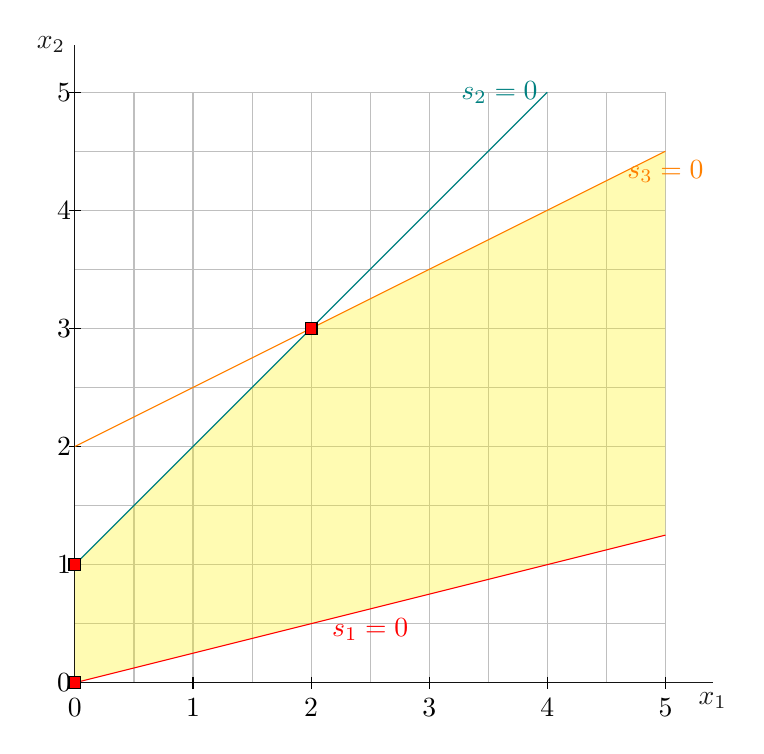
\begin{tikzpicture} [scale=1.5]
    \draw[gray!50, thin, step=.5] (0,0) grid (5,5);
    \draw[opacity=0.9] (0,0) -- (5.4,0) node[below] {$x_1$};
    \draw[opacity=0.9] (0,0) -- (0,5.4) node[left] {$x_2$}; % option \draw[very thick,->]

    \foreach \x in {0,...,5} \draw (\x,0.05) -- (\x,-0.05) node[below] {\x};
    \foreach \y in {0,...,5} \draw (-0.05,\y) -- (0.05,\y) node[left] {\y};

    \fill[yellow,opacity=0.3] (0,0) -- (0,1) -- (2,3) -- (5,4.5) --(5,1.25)-- cycle;

    \draw [red](0,0) -- node[below] {$s_1=0$} (5, 1.25);
    \draw [teal] (0,1)  --  (4,5) node[left, sloped] {$s_2=0$};
    \draw [orange](0,2) --  (5,4.5) node[below, sloped] {$s_3=0$}; %node[above right ,sloped] 
	\filldraw[fill=red] (-0.05,-0.05) rectangle (0.05,0.05);
	\filldraw[fill=red] (-0.05,.95) rectangle (0.05,1.05);
	\filldraw[fill=red] (1.95,2.95) rectangle (2.05,3.05);
\end{tikzpicture} \end{center} 
\end{minipage}

\begin{center}  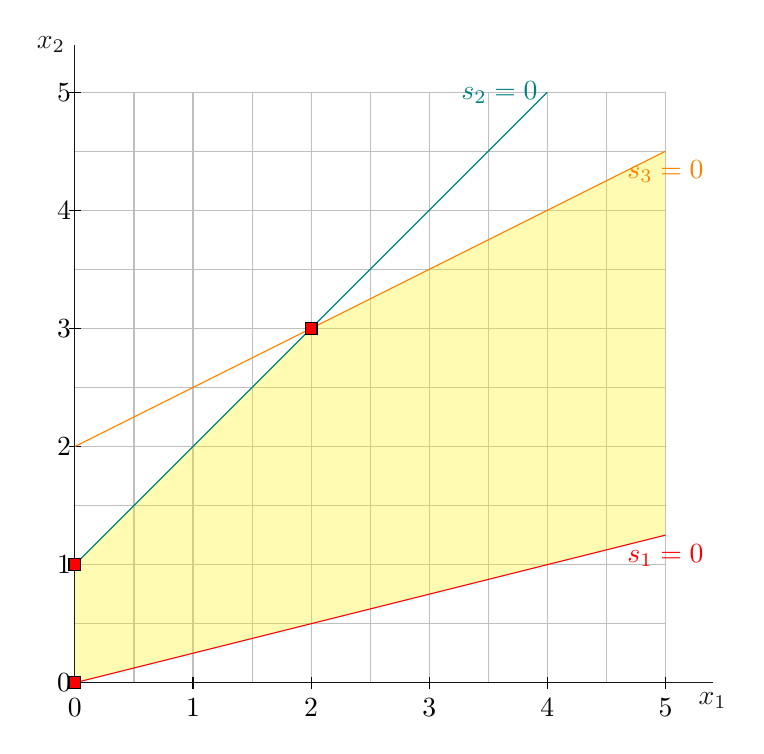
\begin{tikzpicture} [scale=1.5]
    \draw[gray!50, thin, step=.5] (0,0) grid (5,5);
    \draw[opacity=0.9] (0,0) -- (5.4,0) node[below] {$x_1$};
    \draw[opacity=0.9] (0,0) -- (0,5.4) node[left] {$x_2$}; % option \draw[very thick,->]

    \foreach \x in {0,...,5} \draw (\x,0.05) -- (\x,-0.05) node[below] {\x};
    \foreach \y in {0,...,5} \draw (-0.05,\y) -- (0.05,\y) node[left] {\y};

    \fill[yellow,opacity=0.3] (0,0) -- (0,1) -- (2,3) -- (5,4.5) --(5,1.25)-- cycle;

\draw[domain=0:4,smooth,variable=\x, teal] plot ({\x},{\x+1}) node[left] {$s_2=0$};
\draw[domain=0:5,smooth,variable=\x, red] plot ({\x},{\x*1/4}) node[below] {$s_1=0$};
%    \draw [red](0,0) -- node[below] {$s_1=0$} (5, 1.25);
    %\draw [teal] (0,1)  --  (4,5) node[left, sloped] {$s_2=0$};
    \draw [orange](0,2) --  (5,4.5) node[below, sloped] {$s_3=0$}; %node[above right ,sloped] 
	\filldraw[fill=red] (-0.05,-0.05) rectangle (0.05,0.05);
	\filldraw[fill=red] (-0.05,.95) rectangle (0.05,1.05);
	\filldraw[fill=red] (1.95,2.95) rectangle (2.05,3.05);
\end{tikzpicture} \end{center} 

% \draw[scale=0.5,domain=-3:3,smooth,variable=\x,blue] plot ({\x},{\x*\x});


\medskip E.g., consider the $s_3=0$ (orange) line, to find the extreme direction start at extreme point (2,3) and find another feasible point on the orange line, say (4,4) and subtract (2,3) from (4,4), which yields (2,1). 

\medskip This is related to the slope in two-dimensions, as discussed in class, the rise is 1 and the run is 2. So this direction has a slope of 1/2, but this does not carry over easily to higher dimensions where directions cannot be defined by a single number. 

\medskip To find the extreme directions we can change the right-hand-side to $\mathbf{b} = \mathbf{0}$, which forms a polyhedral cone (in yellow), and then add the constraint $x_1 + x_2 = 1$. The intersection of the cone and  $x_1 + x_2 = 1$ form a line segment.

\begin{minipage}[t][][b]{.4\linewidth} \vspace{0mm}
\begin{align*}
\mbox{max~~} & z = -5x_1 - x_2  \\
\mbox{s.t.~~} & x_1 - 4x_2 +s_1 = 0  \\
& -x_1 + x_2 + s_2 = 0 \\
& -x_1 + 2x_2 +s_3 = 0 \\
& x_1 + x_2 = 1 \\
& x_1, x_2, s_1, s_2, s_3 \ge 0.
\end{align*}
\end{minipage}%
\begin{minipage}[t][][b]{.6\linewidth}
\begin{center} 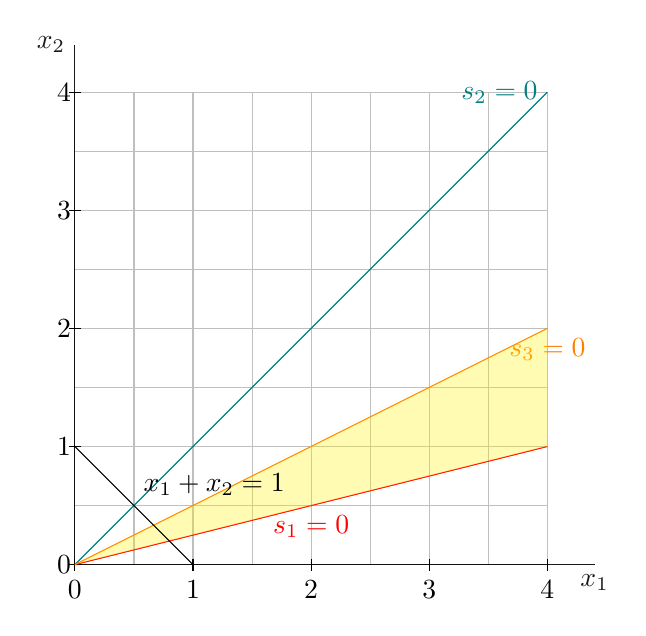
\begin{tikzpicture} [scale=1.5]
\draw[gray!50, thin, step=.5] (0,0) grid (4,4);
\draw[opacity=0.9] (0,0) -- (4.4,0) node[below] {$x_1$};
\draw[opacity=0.9] (0,0) -- (0,4.4) node[left] {$x_2$}; % option \draw[very thick,->]

\foreach \x in {0,...,4} \draw (\x,0.05) -- (\x,-0.05) node[below] {\x};
\foreach \y in {0,...,4} \draw (-0.05,\y) -- (0.05,\y) node[left] {\y};
        
\draw [red](0, 0) -- node[below] {$s_1=0$} (4, 1);
\draw [teal] (0,0)  -- (4,4) node[left, sloped] {$s_2=0$};
\draw [orange](0,0) -- (4,2) node[below, sloped] {$s_3=0$}; 
\fill[yellow,opacity=0.3] (0,0) -- (4,2) -- (4,1) --  cycle; % \draw [orange!50!blue] 

\draw [black] (0,1)  -- node[above right] {$x_1+x_2 = 1$} (1,0); 
\end{tikzpicture} \end{center} 
\end{minipage}



\begin{center} 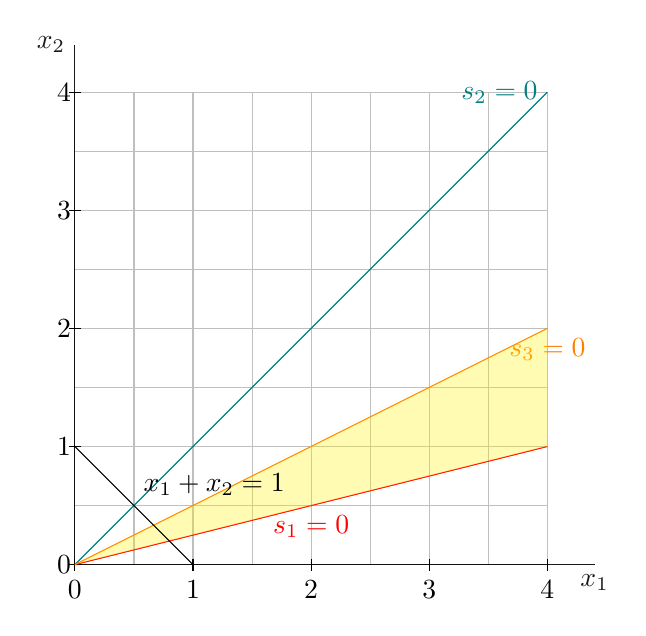
\begin{tikzpicture} [scale=1.5]
\draw[gray!50, thin, step=.5] (0,0) grid (4,4);
\draw[opacity=0.9] (0,0) -- (4.4,0) node[below] {$x_1$};
\draw[opacity=0.9] (0,0) -- (0,4.4) node[left] {$x_2$}; % option \draw[very thick,->]

\foreach \x in {0,...,4} \draw (\x,0.05) -- (\x,-0.05) node[below] {\x};
\foreach \y in {0,...,4} \draw (-0.05,\y) -- (0.05,\y) node[left] {\y};
        
\draw [red](0, 0) -- node[below] {$s_1=0$} (4, 1);
\draw [teal] (0,0)  -- (4,4) node[left, sloped] {$s_2=0$};
\draw [orange](0,0) -- (4,2) node[below, sloped] {$s_3=0$}; 
\fill[yellow,opacity=0.3] (0,0) -- (4,2) -- (4,1) --  cycle; % \draw [orange!50!blue] 

\draw [black] (0,1)  -- node[above right] {$x_1+x_2 = 1$} (1,0); 
\end{tikzpicture} \end{center} 


\medskip Magnifying for clarity, and removing the $s_2=0$ (teal) line, as it is redundant, and marking the extreme points of the new feasible region, (4/5, 1/5) and (2/3, 1/3), with red boxes, we have:

\begin{center}  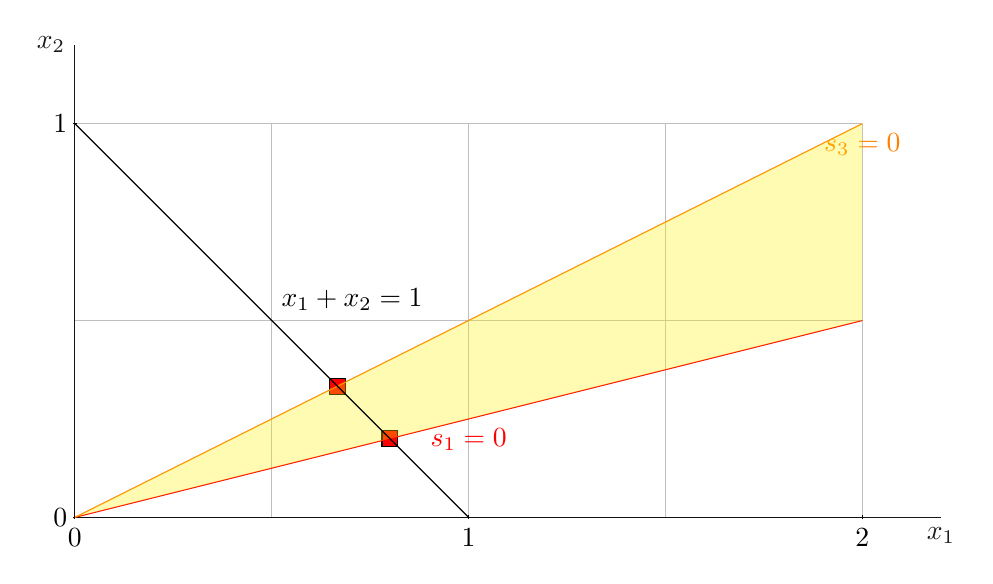
\begin{tikzpicture} [x=50mm, y=50mm] [scale=1.5]
\draw[gray!50, thin, step=.5] (0,0) grid (2,1);
\draw[opacity=0.9] (0,0) -- (2.2,0) node[below] {$x_1$};
\draw[opacity=0.9] (0,0) -- (0,1.2) node[left] {$x_2$}; % option \draw[very thick,->]

\foreach \x in {0,...,2} \draw (\x,0.005) -- (\x,-0.005) node[below] {\x};
\foreach \y in {0,...,1} \draw (-0.005,\y) -- (0.005,\y) node[left] {\y};

\filldraw[fill=red] (0.8-0.02,0.2-0.02) rectangle (0.8+0.02,0.2+0.02);
\filldraw[fill=red] (0.667-0.02,0.333-0.02) rectangle (0.667+0.02,0.333+0.02);

\draw [red](0, 0) -- node[below] {$s_1=0$} (2, .5);
\draw [orange](0,0) -- (2,1) node[below, sloped] {$s_3=0$}; 
\fill[yellow,opacity=0.3] (0,0) -- (2,.5) -- (2,1) --  cycle; % \draw [orange!50!blue] 
\draw [black] (0,1)  -- node[above right] {$x_1+x_2 = 1$} (1,0); 
\end{tikzpicture} \end{center} 

The extreme directions are thus (4/5, 1/5) and (2/3, 1/3). \\

{\bf Representation Theorem:} Let  $\mathbf{x_1}, \mathbf{x_2},\cdots \mathbf{x_k}$ be the set of extreme points of $\mathcal{S}$, and if $\mathcal{S}$ is unbounded, $\mathbf{d_1}, \mathbf{d_2},\cdots \mathbf{d_l}$ be the set of extreme directions. Then any $\mathbf{x} \in \mathcal{S}$ is equal to a convex combination of the extreme points and a non-negative linear combination of the extreme directions: $\mathbf{x} = \sum_{j=1}^k \lambda_j \mathbf{x_j} + \sum_{j=1}^l \mu_j \mathbf{d_j}$, where $\sum_{j=1}^k \lambda_j = 1$, $\lambda_j \ge 0,~\forall  j=1,2,\cdots,k$, and $\mu_j \ge 0,~\forall j=1,2,\cdots,l$.

 \begin{minipage}[t][][b]{.4\linewidth}
\begin{align*}
\mbox{max~~} & z = -5x_1 - x_2  \\\
\mbox{s.t.~~} & x_1 - 4x_2 +s_1 = 0  \\
& -x_1 + x_2 + s_2 = 1 \\
& -x_1 + 2x_2 +s_3 = 4 \\
& x_1, x_2, s_1, s_2, s_3 \ge 0.
\end{align*}
\end{minipage}%
\begin{minipage}[t][][b]{.6\linewidth}
\begin{center}  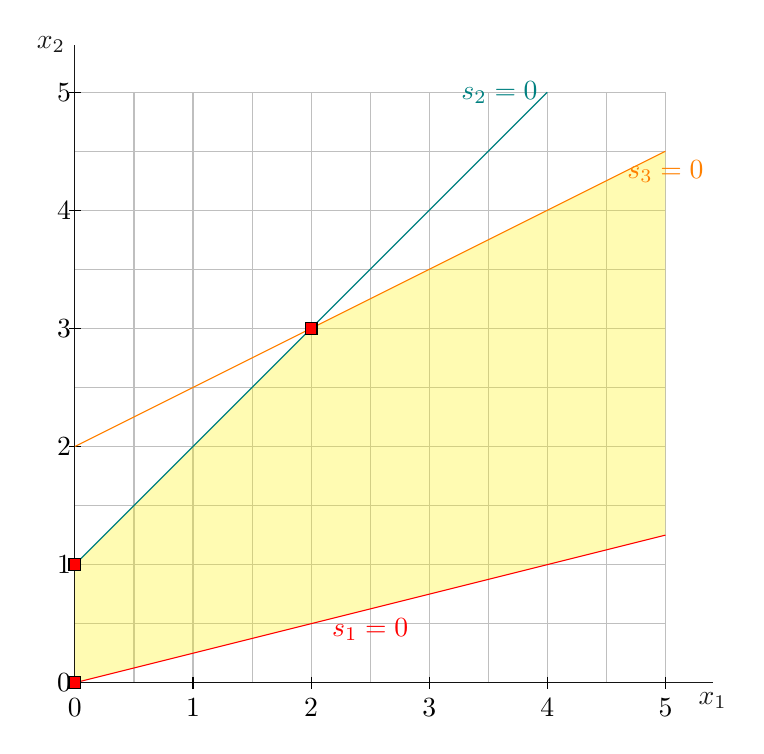
\begin{tikzpicture} [scale=1.5]
    \draw[gray!50, thin, step=.5] (0,0) grid (5,5);
    \draw[opacity=0.9] (0,0) -- (5.4,0) node[below] {$x_1$};
    \draw[opacity=0.9] (0,0) -- (0,5.4) node[left] {$x_2$}; % option \draw[very thick,->]

    \foreach \x in {0,...,5} \draw (\x,0.05) -- (\x,-0.05) node[below] {\x};
    \foreach \y in {0,...,5} \draw (-0.05,\y) -- (0.05,\y) node[left] {\y};

    \fill[yellow,opacity=0.3] (0,0) -- (0,1) -- (2,3) -- (5,4.5) --(5,1.25)-- cycle;

    \draw [red](0,0) -- node[below] {$s_1=0$} (5, 1.25);
    \draw [teal] (0,1)  --  (4,5) node[left, sloped] {$s_2=0$};
    \draw [orange](0,2) --  (5,4.5) node[below, sloped] {$s_3=0$}; %node[above right ,sloped] 
	\filldraw[fill=red] (-0.05,-0.05) rectangle (0.05,0.05);
	\filldraw[fill=red] (-0.05,.95) rectangle (0.05,1.05);
	\filldraw[fill=red] (1.95,2.95) rectangle (2.05,3.05);
\end{tikzpicture} \end{center} 
\end{minipage}

Represent point (1/2, 1) as a convex combination of the extreme points of the above LP.  Find $\lambda$s to solve the following system of equations:

$$\lambda_1 \left[
  \begin{array}{c}
  0 \\
  0 \\
  \end{array} \right]+
 \lambda_2 \left[
  \begin{array}{c}
  0 \\
  1 \\
  \end{array} \right] +
 \lambda_3 \left[
  \begin{array}{c}
  2 \\
  3 \\
  \end{array} \right]  =
 \left[
  \begin{array}{c}
  1/2 \\
  1 \\
  \end{array} \right] 
$$


\newpage The Variable (Canonical Form) and Requirement Space 

\begin{minipage}[t][][b]{.4\linewidth}
\begin{align*}
\mbox{max~~} & z = 2x_1 + x_2  \\\
\mbox{s.t.~~} & x_1 - x_2 +s_1 =  2  \\
& x_1 + x_2 +s_2  = 3 \\
& x_1, x_2, s_1 , s_2  \ge 0.
\end{align*}
\end{minipage}%
\begin{minipage}[t][][b]{.6\linewidth}
\begin{center}  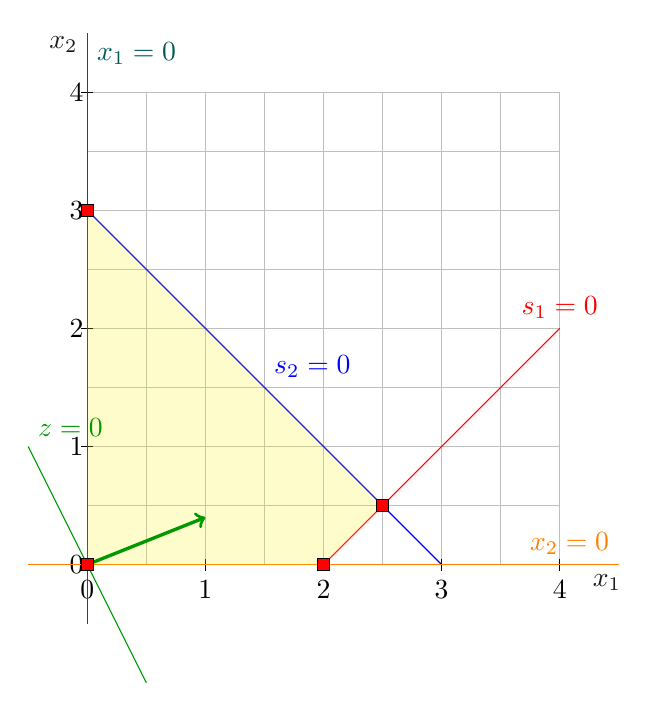
\begin{tikzpicture} [scale=1.5]
\draw[gray!50, thin, step=.5] (0,0) grid (4,4);
\draw[opacity=0.9] (0,0) -- (4.4,0) node[below] {$x_1$};
\draw[opacity=0.9] (0,0) -- (0,4.4) node[left] {$x_2$};

\foreach \x in {0,...,4} \draw (\x,0.05) -- (\x,-0.05) node[below] {\x};
\foreach \y in {0,...,4} \draw (-0.05,\y) -- (0.05,\y) node[left] {\y};

\draw [red](2, 0) --  (4, 2) node[above] {$s_1= 0$};
\draw [blue] (0,3)  -- node[above right] {$s_2=0$} (3,0) ;
\draw [teal!70!black](0,-.5) --  (0,4.5) node[below right] {$x_1=0$}; 
\draw [orange](-.5,0) --  (4.5,0) node[above left] {$x_2=0$}; 

\fill[yellow,opacity=0.2] (0,0) -- (2,0) -- (2.5,0.5) -- (0,3) -- cycle;

\draw [green!60!black] (-0.5, 1)  node[above right] {$z=0$} --  (0.5, -1)  ; % o.f.
\draw [green!60!black, very thick,->](0,0) -- (0+1, 0+2/5); % gradient

\filldraw[fill=red] (-0.05,-0.05) rectangle (0.05,0.05);
\filldraw[fill=red] (2.45,0.45) rectangle (2.55,0.55);
\filldraw[fill=red] (1.95,-0.05) rectangle (2.05,0.05);
\filldraw[fill=red] (-0.05,2.95) rectangle (0.05,3.05);    
\end{tikzpicture} \end{center} 
\end{minipage}



\begin{minipage}[t][][b]{.4\linewidth}
\begin{align*}
\mbox{max~~} & z = 2x_1 + x_2  \\\
\mbox{s.t.~~} & x_1 - x_2 +s_1 =  2  \\
& x_1 + x_2 +s_2  = 3 \\
& x_1, x_2, s_1 , s_2  \ge 0.
\end{align*}
\end{minipage}%
\begin{minipage}[t][][b]{.6\linewidth}
\begin{center}  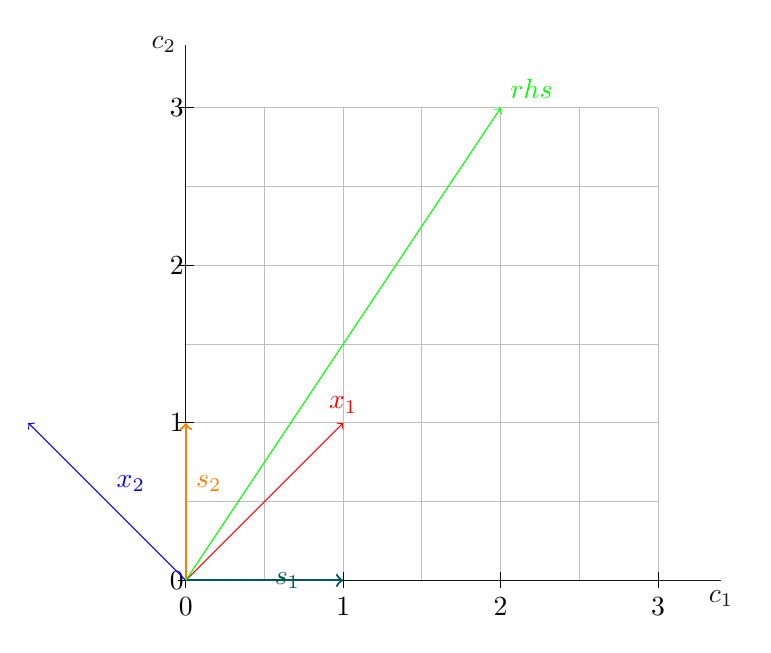
\begin{tikzpicture}[x=20mm, y=20mm] [scale=1.5]  % requirement space
\draw[gray!50, thin, step=.5] (0,0) grid (3,3);
\draw[opacity=0.9] (0,0) -- (3.4,0) node[below] {$c_1$};
\draw[opacity=0.9] (0,0) -- (0,3.4) node[left] {$c_2$};

\foreach \x in {0,...,3} \draw (\x,0.05) -- (\x,-0.05) node[below] {\x};
\foreach \y in {0,...,3} \draw (-0.05,\y) -- (0.05,\y) node[left] {\y};

\draw [red,->](0, 0) --  (1, 1) node[above] {$x_1$};
\draw [blue,->] (0,0)  -- node[above right] {$x_2$} (-1,1) ;
\draw [thick, teal!70!black,->](0,0) -- node[right] {$s_1$} (1,0); 
\draw [thick, orange,->](0,0) -- node[above right] {$s_2$} (0,1); 
\draw [green,->] (0, 0)  --  (2,3) node[above right] {$rhs$}   ; 
\end{tikzpicture} \end{center} 
\end{minipage}


\newpage \underline {\bf Tableaus} \\  % introducing tableaus

After putting an LP into standard form, we can put the system of equations into a table form, the ``tableau". \\

\begin{minipage}[t][][b]{.4\linewidth} \vspace{-5mm}
\begin{align*}
\mbox{max~~} & z = 2x_1 + x_2  \\
\mbox{s.t.~~} & x_1 - x_2 +s_1 =  2  \\
& x_1 + x_2 +s_2  = 3 \\
& x_1, x_2, s_1 , s_2  \ge 0.
\end{align*}
\end{minipage}%
\begin{minipage}[t][][b]{.6\linewidth}
\begin{center} \begin{tabular} {l|c||c|c|c|c|c|}  \cline{2-7}
max & $z$	& $x_1$ & $x_2$  & $x_3$	& $x_4$	& $rhs$ \\ \cline{2-7}
(r0 - z)	    & 1		& -2        &  -1        &	 0 	    &	  0		&   0    \\ \cline{2-7}
(r1 - $x_3$)			& 0		&	 1        &     -1     &	 1 			&	  0 		&	  2   \\
(r2 - $x_4$)			& 0		&	  1       &	    1    &	 0 		&	  1 		&	   3   \\ \cline{2-7}
\end{tabular} \end{center}
\end{minipage} \\
 
\bigskip Why are the coefficients negative in row zero, we change $z = 2x_1 + x_2 $ to $z - 2x_1 - x_2 =0$ so we have only constants on the right-hand-side (rhs). \\

This tableau represents a basic solution, because it contains an identity matrix.  The basic variables are those variables having columns in the identity matrix (here, $x_3$ and $x_4$), and it is feasible because the rhs for row $1-m$ are non-negative. \\

We can consider $z$ a permanent member of an expanded basis if we treat row zero like any other row (although the rhs of row~0 can be negative).

\newpage \underline{\bf Basic Solutions and Extreme Points}

\begin{minipage}[t][][b]{.55\linewidth} \vspace{2mm}
\begin{center} \begin{tabular} {l|c||c|c|c|c|c|}  \cline{2-7}
max & $z$	& $x_1$ & $x_2$  & $x_3$	& $x_4$	& $rhs$ \\ \cline{2-7}
(r0 - z)	    & 1		& -2        &  -1        &	 0 	    &	  0		&   0    \\ \cline{2-7}
(r1 - $x_3$)			& 0		&	 1        &     -1     &	 1 			&	  0 		&	  2   \\
(r2 - $x_4$)			& 0		&	  1       &	    1    &	 0 		&	  1 		&	   3   \\ \cline{2-7}
\end{tabular} \end{center}
\end{minipage}%
\begin{minipage}[t][][b]{.45\linewidth}
\begin{center}  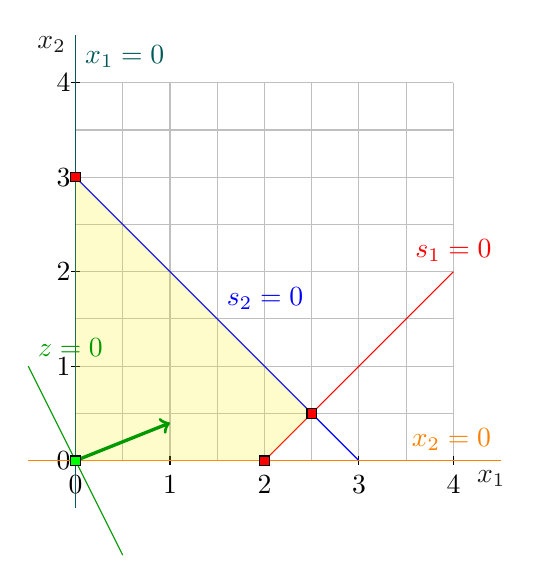
\begin{tikzpicture} [scale=1.2]
\draw[gray!50, thin, step=.5] (0,0) grid (4,4);
\draw[opacity=0.9] (0,0) -- (4.4,0) node[below] {$x_1$};
\draw[opacity=0.9] (0,0) -- (0,4.4) node[left] {$x_2$};

\foreach \x in {0,...,4} \draw (\x,0.05) -- (\x,-0.05) node[below] {\x};
\foreach \y in {0,...,4} \draw (-0.05,\y) -- (0.05,\y) node[left] {\y};

\draw [red](2, 0) --  (4, 2) node[above] {$s_1= 0$};
\draw [blue] (0,3)  -- node[above right] {$s_2=0$} (3,0) ;
\draw [teal!70!black](0,-.5) --  (0,4.5) node[below right] {$x_1=0$}; 
\draw [orange](-.5,0) --  (4.5,0) node[above left] {$x_2=0$}; 

\fill[yellow,opacity=0.2] (0,0) -- (2,0) -- (2.5,0.5) -- (0,3) -- cycle;

\draw [green!60!black] (-0.5, 1)  node[above right] {$z=0$} --  (0.5, -1)  ; % o.f.
\draw [green!60!black, very thick,->](0,0) -- (0+1, 0+2/5); % gradient

\filldraw[fill=green] (-0.05,-0.05) rectangle (0.05,0.05);
\filldraw[fill=red] (2.45,0.45) rectangle (2.55,0.55);
\filldraw[fill=red] (1.95,-0.05) rectangle (2.05,0.05);
\filldraw[fill=red] (-0.05,2.95) rectangle (0.05,3.05);    
\end{tikzpicture} \end{center} 
\end{minipage}

Here the basic variables are $x_3 = 2$ and $x_4=3$, and the $z$-value of objective function value is 0. \\

Let's go to the extreme point (2,0) which has basic variables $x_1$ and $x_4$ (this new extreme point is adjacent to the extreme point (0,0). Why? \\
% they share an edge, and are defined by the same n-1 hypeplanes.
\begin{center} \begin{tabular} {l|c||c|c|c|c|c|}  \cline{2-7}
max & $z$	& $x_1$ & $x_2$  & $x_3$	& $x_4$	& $rhs$ \\ \cline{2-7}
(r0 - z)	    & 1		& -2        &  -1        &	 0 	    &	  0		&   0    \\ \cline{2-7}
(r1 - $x_3$)			& 0		&	 1        &     -1     &	 1 			&	  0 		&	  2   \\
(r2 - $x_4$)			& 0		&	  1       &	    1    &	 0 		&	  1 		&	   3   \\ \cline{2-7}
\end{tabular} \end{center}

First get a 1 coefficent in row~1 in the  $x_1$ column by multiplying row~1 by a scalar (no action needed, already equals one).\\
 
\begin{center} \begin{tabular} {l|c||c|c|c|c|c|}  \cline{2-7}
max 			& $z$	& $x_1$ & $x_2$  & $x_3$	& $x_4$	& $rhs$ \\ \cline{2-7}
(r0 - z)	    & 1		& -2        &  -1        &	 0 	    &	  0		&   0    \\ \cline{2-7}
(r1 - $x_3$)	& 0		&	 1        &     -1     &	 1 			&	  0 		&	  2   \\
(r2 - $x_4$)	& 0		&	  1       &	    1    &	 0 		&	  1 		&	   3   \\ \cline{2-7}
\end{tabular} \end{center}

Then use row~1 to zero out the row~0 coefficient for $x_1$ by multiplying row~1 by 2 and adding it to row~0 to get a new row~0.\\


\begin{center} \begin{tabular} {l|c||c|c|c|c|c|}  \cline{2-7}
max 			& $z$	& $x_1$ & $x_2$  & $x_3$	& $x_4$	& $rhs$ \\ \cline{2-7}
(r0 -z)	    	& 1		& 0     & -3     &	 2 	&	  0	&   4    \\ \cline{2-7}
(r1 - $x_3$)	& 0		& 1     & -1     &	 1 	&	  0 &	  2   \\
(r2 - $x_4$)	& 0		& 1     &  1    &	 0 	&	  1 &	   3   \\ \cline{2-7}
\end{tabular} \end{center}

Lastly use row~1 to zero out the row~20 coefficient for $x_1$ by multiplying row~1 by -1 and adding it to row~2 to get a new row 2. \\


\begin{center} \begin{tabular} {l|c||c|c|c|c|c|}  \cline{2-7}
max 			& $z$	& $x_1$ & $x_2$  & $x_3$	& $x_4$	& $rhs$ \\ \cline{2-7}
(r0 -z)	    	& 1		& 0     & -3     &	 2 	&	  0	&   4    \\ \cline{2-7}
(r1 - $x_3$)	& 0		& 1     & -1     &	 1 	&	  0 &	2   \\
(r2 - $x_4$)	& 0		& 0     &  2    &	-1 	&	  1 &	1   \\ \cline{2-7}
\end{tabular} \end{center}

\newpage The nonbasic variables for this tableau are $x_2$ and $x_3$, so we can graph the new LP in the nonbasic variable space.

\begin{minipage}[t][][b]{.55\linewidth} \vspace{2mm}
\begin{center} \begin{tabular} {l|c||c|c|c|c|c|}  \cline{2-7}
max 			& $z$	& $x_1$ & $x_2$  & $x_3$	& $x_4$	& $rhs$ \\ \cline{2-7}
(r0 -z)	    	& 1		& 0     & -3     &	 2 	&	  0	&   4    \\ \cline{2-7}
(r1 - $x_3$)	& 0		& 1     & -1     &	 1 	&	  0 &	2   \\
(r2 - $x_4$)	& 0		& 0     &  2    &	-1 	&	  1 &	1   \\ \cline{2-7}
\end{tabular} \end{center}
\end{minipage}%
\begin{minipage}[t][][b]{.45\linewidth}
\begin{center}  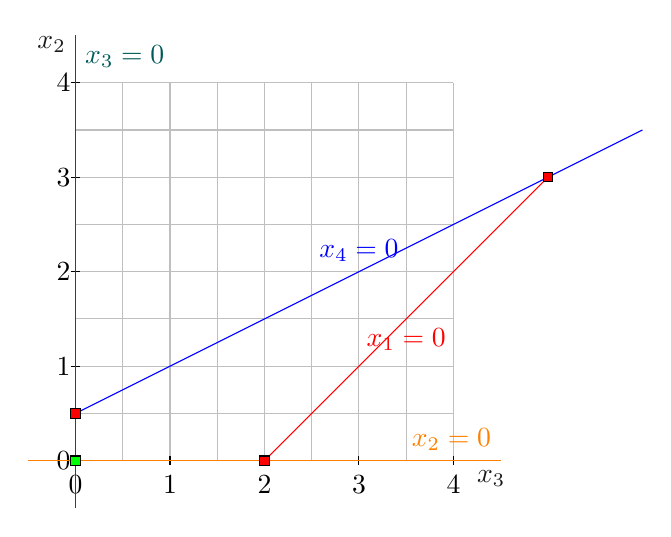
\begin{tikzpicture} [scale=1.2]
\draw[gray!50, thin, step=.5] (0,0) grid (4,4);
\draw[opacity=0.9] (0,0) -- (4.4,0) node[below] {$x_3$};
\draw[opacity=0.9] (0,0) -- (0,4.4) node[left] {$x_2$};

\foreach \x in {0,...,4} \draw (\x,0.05) -- (\x,-0.05) node[below] {\x};
\foreach \y in {0,...,4} \draw (-0.05,\y) -- (0.05,\y) node[left] {\y};

\draw [red](2, 0) --  node[below] {$x_1= 0$} (5, 3) ;
\draw [blue] (0,0.5)  -- node[above] {$x_4=0$} (6,3.5) ;
\draw [teal!70!black](0,-.5) --  (0,4.5) node[below right] {$x_3=0$}; 
\draw [orange](-.5,0) --  (4.5,0) node[above left] {$x_2=0$}; 

%\fill[yellow,opacity=0.2] (0,0) -- (2,0) -- (2.5,0.5) -- (0,3) -- cycle;

%\draw [green!60!black] (-0.5, 1)  node[above right] {$z=0$} --  (0.5, -1)  ; % o.f.
%\draw [green!60!black, very thick,->](0,0) -- (0+1, 0+2/5); % gradient

\filldraw[fill=green] (-0.05,-0.05) rectangle (0.05,0.05);
\filldraw[fill=red] (1.95,-0.05) rectangle (2.05,0.05);
\filldraw[fill=red] (4.95,2.95) rectangle (5.05,3.05);
\filldraw[fill=red] (-0.05,0.45) rectangle (0.05,0.55);    
\end{tikzpicture} \end{center} 
\end{minipage}



\newpage \underline{\bf Matrix Math}

\bigskip  An $m \times n$ matrix is an array of real numbers with $m$ rows and $n$ columns. Any matrix can be represented by its constituent set of row or column vectors. \\

$\mathbf{A} =
\left[
  \begin{array}{cc}
    1 & 3 \\
    6 & 4 \\
  \end{array}
\right]     =
\left[
  \begin{array}{cc}
  \mathbf{a_1} & \mathbf{a_2} \\
  \end{array}
\right]     =
\left[
  \begin{array}{c}
  \mathbf{a^1} \\
  \mathbf{a^2} \\
  \end{array}
\right], $ \\

\noindent where
$\mathbf{a_1} =
\left[
  \begin{array}{c}
  1 \\
  6 \\
  \end{array}
\right],~ \mathbf{a_2} =
\left[
  \begin{array}{c}
  3 \\
  4 \\
  \end{array} \right],~
\mathbf{a^1} =
\left[\begin{array}{cc}
  1 & 3 \\
\end{array} \right],~ $and$~
\mathbf{a^2} = \left[\begin{array}{cc}
  6 & 4 \\
\end{array} \right]$.  Additionally, $a_{11} = 1$, $a_{12} = 3$, $a_{21} = 6$, $a_{22} = 4$. \\

{\bf Matrix Addition:} Two matrices of the same dimension can be added componentwise, thus $\mathbf{C} = \mathbf{A} + \mathbf{B}$ means that $c_{ij} = a_{ij} + b_{ij}$. \\

{\bf Scalar Multiplication:} Just like it sounds. If $k$ is a scalar, then $k\mathbf{A}$ means that every component of $\mathbf{A}$ is multiplied by $k$. \\

{\bf Matrix Multiplication:} $\mathbf{A}$ is a $m \times n$ matrix and $\mathbf{B}$ is a $p \times q$ matrix.  $\mathbf{AB}$ (matrix multiplication) is only defined if $n = p$ and the result is a $m \times q$ matrix, $\mathbf{BA}$ is only defined if $q = m$ and the result is a $p \times n$. $\mathbf{AB}$ is not necessarily equal to $\mathbf{BA}$, thus $\mathbf{C} = \mathbf{AB}$ where $c_{ij} = \sum_{k=1}^n a_{ik}b_{kj},~ i=1,\cdots,m,~ j=1,\cdots,p$, e.g., $c_{11}$ is the sum of the the componentwise multiplication of the first row of $\mathbf{A}$ and the first column of $\mathbf{B}$. \\

{\bf Identity Matrix:} A square matrix (denoted by $\mathbf{I}$) with all zero components, except for the diagonal: \\
$\left[ \begin{array}{ccc}
     1 & 0 & 0 \\
     0 & 1 & 0 \\
     0 & 0 & 1 \\
\end{array} \right]$ \\


{\bf Elementary Matrix Operations:}
These operations are used to solve systems of linear equations or inverting a matrix. The three operations are as follows (for any matrix $\mathbf{A}$):

\begin{itemize}
\item Interchange two rows of $\mathbf{A}$.
\item Multiply a row by a nonzero scalar.
\item Replace row $i$ with row $i$ plus row $j$ multiplied by a nonzero scalar.
\end{itemize}

\bigskip {\bf Inverting a Matrix:}

\bigskip $\mathbf{A} = \left[
   \begin{array}{ccc}
     3 & 9 & 2 \\
     1 & 1 & 1 \\
     5 & 4 & 7 \\
   \end{array} \right]~and~\mathbf{A^{-1}} = \left[
   \begin{array}{ccc}
     -\frac{3}{11} & 5 & -\frac{7}{11} \\
     \frac{2}{11} & -1 & \frac{1}{11} \\
     \frac{1}{11} & -3 & \frac{6}{11} \\
   \end{array} \right]$

\bigskip To find $\mathbf{A^{-1}}$ using elementary row operations to transform $\mathbf{A}$ into an identity matrix, while performing these same operations on the attached identity matrix.

\bigskip $\left[ \begin{array}{ccc|ccc} \nonumber
         3 & 9 & 2 & 1 & 0 & 0 \\
         1 & 1 & 1 & 0 & 1 & 0 \\
         5 & 4 & 7 & 0 & 0 & 1 \\
\end{array} \right] \Rightarrow
\left[ \begin{array}{ccc|ccc} \nonumber
         1 & 0 & 0 & -\frac{3}{11} & 5 & -\frac{7}{11} \\
         0 & 1 & 0 & \frac{2}{11} & -1 & \frac{1}{11} \\
         0 & 0 & 1 & \frac{1}{11} & -3 & \frac{6}{11} \\
\end{array} \right].$ \\

{\bf Rank of a Matrix:} $\mathbf{A}$ is a $m \times n$ matrix then rank$(\mathbf{A}) \le min\{m,~n\}$, if rank$(\mathbf{A}) = min\{m,~n\}$, then $\mathbf{A}$ is of full rank.  If $\mathbf{A}$ is not full rank, but of rank $k$, where $k < min\{m,~n\}$, then using the elementary row operations, we can transform $\mathbf{A}$ to the following:
$\left[
   \begin{array}{cc}
     \mathbf{I_k} & \mathbf{Q}  \\
     0            & 0 \\
\end{array} \right]$

\begin{comment}
\bigskip {\bf Simultaneous Linear Equations}

\bigskip Consider the system $\mathbf{A} \mathbf{x} = \mathbf{b}$, where $\mathbf{A}$ is a $m \times n$ matrix of rank $m$ and $m \le n$. We can partition $\mathbf{A}$ such that $\mathbf{A} = [\mathbf{B}, \mathbf{N}]$, where
\begin{itemize}
\item the {\it basis matrix} $\mathbf{B}$ is a nonsingular (i.e., it consists of $m$ linearly dependent columns of $\mathbf{A}$) $m \times m$ matrix.
\item the {\it nonbasic matrix} $\mathbf{N}$ is a $m \times n-m$ matrix
\end{itemize}

The vector $\mathbf{x}$ can be divided in a similar way (each column corresponds to a variable), yielding $\mathbf{x_B}$ and $\mathbf{x_N}$. \\

We can write our system as follows: 
$$\mathbf{B} \mathbf{x_B} + \mathbf{N} \mathbf{x_N} = \mathbf{b}.$$ 
$$\mathbf{B} \mathbf{x_B}  = \mathbf{b}-  \mathbf{N} \mathbf{x_N}.$$ 
Premultiplying by $\mathbf{B^{-1}}$ yields:  
$$\mathbf{x_B} = \mathbf{B^{-1}}\mathbf{b} - \mathbf{B^{-1}} \mathbf{N} \mathbf{x_N}.$$ 

By setting $\mathbf{x_N} = \mathbf{0}$ and solving we (potentially) find a {\it basic feasible solution} to the system, which corresponds to an extreme point of the feasible region, remember that the nonbasic variables $\mathbf{x_N} = \mathbf{0}$ represent the defining hyperplanes for a solution. For any set of $m$ variables, the result can be:

\begin{enumerate}
\item a basic feasible solution, $\mathbf{x_B} \ge \mathbf{0}$.
\item a basic infeasible solution, some $x \in \mathbf{x_B} \le 0$.
\item a set of linearly dependent columns that does not span the $m$-space.
\end{enumerate}

For this system there are possibly ${n \choose m}$ basic solutions, that is, the number of basic feasible solutions is bounded by $n!/m!(n-m)!$ from above.  \\




\bigskip The following are the four possible cases for an LP:
%Describe (0.5, 1) in terms of extreme points and directions.
%Describe (3, 2) in terms of extreme points and directions.



\begin{itemize}
\item Unique optimal solution 
\item Multiple optimal solutions
\item Unbounded optimal objective value
\item Empty feasible region (an infeasible LP)
\end{itemize}
\end{comment}